\documentclass[tese-proposta,nocipinfo]{texufpel}
%nocipinfo para não aparecer os dados da CIP no Resumo

\usepackage[utf8]{inputenc} % acentuacao
\usepackage{graphicx} % para inserir figuras
\usepackage[T1]{fontenc}
\usepackage{hyperref}
\usepackage{verbatim}
\usepackage{makecell}
\usepackage{enumitem}
\usepackage{cleveref}


\hypersetup{
    hidelinks, % Remove coloração e caixas
    unicode=true,   %Permite acentuação no bookmark
    linktoc=all %Habilita link no nome e página do sumário
}

\unidade{Centro de Desenvolvimento Tecnológico}
\programa{Programa de Pós-Graduação em Computação}
\curso{Ciência da Computação}

\title{Exploração Precoce do Espaço de Projeto:\\Aplicando Heurísticas e Simulação em Nível de Sistema na Avaliação\\de Cargas de Trabalho sobre Arquiteturas Heterogêneas}


%\title{Exploração Precoce do Espaço de Projeto:\\Usando Heurísticas de Seleção de Soluções Candidatas e Simulação em Nível de Sistema na Análise de Cargas de Trabalho Específicas sobre Arquiteturas Multiprocessadas Heterogêneas durante as Fases Iniciais no Desenvolvimento de Sistemas Embarcados}

%\title{Exploração do Espaço de Projeto em Fases Iniciais de Desenvolvimento Visando o Aumento da Heterogeneidade de Sistemas Embarcados}
%: Uso de Modelos Abstratos de Aplicações e Arquitetura na Simulação em Nível de Sistemas Considerando Paralelismo em Nível de Tarefa e Detalhes de Uso de Memória}
%\title{Aumentando a Heterogeneidade de Sistemas usando o Paralelismo de Nível de Tarefa e considerando Detalhes de Uso de Memória}

\author{Betemps}{Carlos Michel}
\advisor[Prof.~Dr.]{Zatt}{Bruno}
\coadvisor[Prof.~Dr.]{Palomino}{Daniel Munari Vilchez}
\coadvisor[Prof.~Dr.]{Porto}{Marcelo Schiavon}
%\collaborator[Prof.~Dr.]{Porto}{Marcelo Schiavon}


%Palavras-chave em PT_BR
\keyword{Exploração do Espaço de Projeto}
%\keyword{Heurísticas e Meta-heurísticas}
\keyword{Heurísticas}
\keyword{Modelos em Alto Nível de Abstração}
\keyword{Paralelismo em Nível de Tarefa}
\keyword{Heterogeneidade}
\keyword{Sistemas Embarcados}

%Palavras-chave em EN_US
\keywordeng{Design Space Exploration (DSE)}
%\keywordeng{Heuristics and Metaheuristics}
\keywordeng{Heuristics}
\keywordeng{High-Abstraction Level Models}
\keywordeng{Task-level Parallelism}
\keywordeng{Heterogeneity}
\keywordeng{Embedded Systems}

\begin{document}
\newcommand{\Topico}{\textcolor{red}{>>}\textcolor{red}}
%\renewcommand{\advisorname}{Orientadora}           %descomente caso tenhas orientadora
%\renewcommand{\coadvisorname}{Coorientadora}      %descomente caso tenhas coorientadora

\makeatletter
\newcommand\footnoteref[1]{\protected@xdef\@thefnmark{\ref{#1}}\@footnotemark}
\makeatother

\maketitle 
\sloppy


%%%%%%%%%%%%%%%%%%%%%%%%%%%%%%%%%%%%%%%%%%%%%%%%%%%%%%%%
%%%%%%%%%%%%%%%%%     Resumo   %%%%%%%%%%%%%%%%%%%%%%%%%
%%%%%%%%%%%%%%%%%%%%%%%%%%%%%%%%%%%%%%%%%%%%%%%%%%%%%%%%
%Resumo em Portugues (no maximo 1 pagina)
%Apresentar aqui uma breve Introdução ao Problema que está se pretendendo resolver ou abordar. Além disso, nesta Seção, apresenta(m)-se o(s) principal(is) objetivo(s) do projeto e, portanto, a(s) principal(is) contribuição(ções).
%\Topico{Exploração do Espaço de Projeto em fases iniciais de Desenvolvimento} \Topico{Aumento da Heterogeneidade de Sistemas} \Topico{Contribuições}
\begin{abstract}



\end{abstract}


\begin{comment}
Roteiro para elaboração de uma Proposta de Dissertação ou de Tese

Este é um modelo que irá ajudá-lo a preparar o seu Projeto de Dissertação ou Tese. A ideia é não utilizar este roteiro como um esqueleto para o texto, mas garantir que estas informações estejam disponíveis. Lembrar que deve ficar claro o que será realizado e o que este resultado traz em adição aos trabalhos em curso ou já documentados na literatura.
O texto deve transparecer o domínio do aluno sobre o tema. Isso não quer dizer que ele deva apresentar uma revisão bibliográfica sobre o tema, mas deve sim ter o poder de síntese, expressando aspectos relevantes dos trabalhos relacionados e do próprio tema de pesquisa a serem considerados no seu próprio trabalho.

1. Histórico e Temática do Estudo
Apresentar o tema de estudo, delimitando áreas e subáreas da Computação e informações históricas.

2. Caracterização do Problema
De forma resumida, apresentar o contexto do trabalho, o principal objetivo a ser obtido, a forma de avaliação e a contribuição a ser dada.

3. Justificativa
    a. Relevância: Descrever a relevância do tema para a comunidade em geral, qual a contribuição da área para a sociedade como um todo.
    b. Contribuição: Quais são os aspectos não tratados em trabalhos relacionados/anteriores. Qual o avanço do estado da arte. 

4. Contexto do Trabalho
Trabalhos relacionados e abordagens apresentadas. Emergir os aspectos de pesquisa relacionados.

5. Objetivos
Apresentar de forma clara e precisa o objetivo, ou os objetivos se for o caso, a ser atingido e as metas a serem cumpridas para alcançá-lo.

6. Base de Desenvolvimento
Caracterizar os recursos a serem utilizados no desenvolvimento do trabalho, tanto aquele caracterizando o referencial teórico, como o ferramental necessários.

7. Metodologia
    a. De desenvolvimento: Descrição do tratamento que será dado ao referencial teórico e como as ferramentas serão utilizadas.
    b. De validação dos resultados: Como os resultados serão avaliados e comparados/contrastados com os apresentados na literatura.

8. Cronograma
Listagem das atividades, com breve descrição e identificação dos resultados a serem obtidos em cada uma. Distribuição no tempo. Granularidade: mensal. Dependência temporal entre elas.

9. Resultados Esperados
Discutir os veículos de divulgação, conferências, revistas etc, especializadas no tema e identificar aquelas que poderão ser alvo de submissão de trabalhos.

10. Referencial Bibliográfico
Citadas nesta proposta.



Retalhos:::
\chapter{Motivação}
% (ENTRE 1 e 2 PÁGINAS)
%Nesta Seção, apresenta-se um breve histórico da área de concentração da Tese, partindo do tema mais abrangente até chegar especificamente no assunto do Projeto. Além disso, apresenta-se a justificativa para a realização do trabalho, sua importância acadêmica ou para comunidade e grau de inovação. Poderá também apresentar as distinções entre o trabalho atual e outros trabalhos já realizados.
%A área de concentração da tese é apresentada nesta seção, abordando o domínio de Sistemas Embarcados e seu desenvolvimento, passando pelo tema de heterogeneidade dos sistemas atuais de computação e o uso de simulação em nível de sistema como uma forma de avaliar o comportamento e interações do sistema em desenvolvimento durante fases iniciais de projeto. \Topico{Heurística}. \Topico{DSE}. Finalmente, trabalhos atuais relacionados são abordados ressaltando os aspectos que poderiam ser melhorados, os quais deverão ser atacados pelo trabalho ora proposto.


\end{comment}


%%%%%%%%%%%%%%%%%%%%%%%%%%%%%%%%%%%%%%%%%%%%%%%%%%%%%%%%
%%%%%%%%%%%     Capítulo ou Seção   %%%%%%%%%%%%%%%%%%%%
%%%%%%%%%%%%%%%%%%%%%%%%%%%%%%%%%%%%%%%%%%%%%%%%%%%%%%%%
\chapter{Introdução e Motivação}
Sistemas Embarcados (SE) implementam funções dedicadas e específicas dentro de um sistema hospedeiro \cite{Camposano1996}. São componentes de sistemas maiores usados para controlar e/ou diretamente monitorar tais sistemas \cite{Guessi:2012:ArchitecturalDescription}. Podem ser considerados como sistemas de processamento de informações que estão embarcadas em um produto maior e que normalmente não são diretamente visíveis para o usuário \cite{marwedel2006embedded}.

SEs são altamente diversos, variando desde pequenos sistemas como refrigeradores, máquinas de auto-atendimento ou sensores inteligentes em automação de construções até sistemas distribuídos e complexos como sistemas de controle automotivo e aeroespacial \cite{Voelter2013}. Software embarcado também está em constante crescimento quanto as funcionalidades implementadas, tamanho e complexidade \cite{Hendriks2016}. Assim, o projeto de SEs está em um contexto altamente competitivo e que evolui rapidamente a medida que novas tecnologias são introduzidas \cite{bertels2012HW:SW:Introduction}. A transformação de um projeto (\textit{design}) eficiente em um produto de sucesso depende do mesmo se tornar o primeiro no mercado (\textit{time-to-market}), proporcionando novas funcionalidades (primeiro produto a prover tais funcionalidades), obedecendo às restrições de desempenho e a um preço acessível \cite{Herrera201455, mischkalla2010closing}.

O projeto de SEs (sistemas de hardware e software) normalmente envolve modelagem, validação e implementação \cite{DeMicheli_Gupta1997}. A \textbf{modelagem} trata da conceitualização e refinamento das especificações, produzindo modelos de hardware e software. A \textbf{validação} busca o alcance de um nível de confiança razoável de que o sistema funcionará como projetado. A \textbf{implementação} é a realização física do hardware e do software.

Devido à complexidade do projeto de novos produtos, a competitividade no mercado de SEs, e a lacuna existente no projeto conjunto de hardware e software, cada vez mais tarefas de exploração de alternativas de soluções são realizadas em nível de sistema \cite{gries2004methods,gajski2009embedded}, de forma a possibilitar a tomada de decisões em fases iniciais de desenvolvimento. Neste contexto, são utilizados modelos em alto nível de abstração para descrever as diferentes configurações de arquitetura e as cargas de trabalho a serem submetidas ao sistema. Como as avaliações precisam ocorrer em fases iniciais de desenvolvimento, quando normalmente ainda não há disponibilidade de arquitetura e de aplicações que possam ser executadas, a utilização de simulação em nível de sistema surge como alternativa para avaliação de soluções durante a Exploração do Espaço de Projeto (DSE - \textit{Design Space Exploration}). 

Exploração do Espaço de Projeto (DSE - \textit{Design Space Exploration}) é o processo de analisar o conjunto de possíveis soluções e definir qual será selecionada \cite{marwedel2006embedded}. O desempenho de um sistema depende de um conjunto diverso de fatores, tais como arquitetura da aplicação de software, arquitetura da plataforma de hardware, de como as funcionalidades da aplicação são executadas pelos elementos de processamento (como CPUs, GPUs, FPGAs, ASICs, DSPs, etc.), além de vários parâmetros tais como tamanhos de caches, tamanho de memória, dentre outros. Isto faz da DSE uma atividade chave para permitir avaliações do sistema logo no início das iniciativas de desenvolvimento \cite{Herrera201455}. De forma geral, uma abordagem de DSE consiste de quatro componentes básicos \cite{Ascia2011382}: (\textit{i}) um ponto de entrada representado pela(s) configuração(ões) inicial(ais), (\textit{ii}) um modelo de avaliação das configurações, (\textit{iii}) estratégia de exploração que consiste de um conjunto de transformações a serem aplicadas nas configurações e (\textit{iv}) um critério de parada. 


Normalmente, o processo de DSE segue a abordagem \textit{Y-chart} \cite{gries2004methods}. Nesta abordagem, um modelo de aplicação (ou aplicações -- a carga de trabalho a ser submetida ao sistema) -- derivado a partir do domínio da aplicação alvo -- descreve o seu comportamento funcional de uma maneira independente de arquitetura. Simultaneamente, um modelo de arquitetura -- definido considerando a aplicação -- define os recursos da arquitetura (elementos de processamento - PE (\textit{processing elements})) e captura suas restrições de desempenho \cite{Jia:2013:NASAFramework}. Ademais, ambos modelos são considerados, de forma separada, e um terceiro modelo -- de \textbf{mapeamento} -- define uma ligação entre ambos (cada tarefa da aplicação é alocada para execução em um determinado PE da arquitetura) \cite{gries2004methods}. O modelo de mapeamento mapeia o modelo de aplicação no modelo de arquitetura para execução (por meio de co-simulação, por exemplo), depois do qual distintas métricas de sistema podem ser quantitativamente avaliadas \cite{Jia:2013:NASAFramework}. A abordagem \textit{Y-chart} consiste \cite{gries2004methods}, basicamente, do mapeamento entre a carga de trabalho (\textit{workload}) e os elementos de processamento da arquitetura. Após, considerando métricas como, por exemplo, desempenho e dissipação de potência, é realizada a \textbf{análise} das configurações em investigação por meio de testes que podem incluir execução em hardware real, simulação ou geração de estimativas. As \textbf{métricas} de desempenho são utilizadas como base para proceder com ajustes na arquitetura, nas aplicações ou mesmos nos mapeamentos. A Fig. \ref{fig:y-chart} ilustra os passos da referida abordagem. 
%Os desafios básicos de um processo de DSE são \cite{chakraverty2014fuzzy}: \textit{seleção dos recursos} - que unidades de processamento e links de comunicação serão utilizados; \textit{atribuição de tarefas} (\textit{task assignment}) - distribuir as tarefas de uma aplicação entre os recursos selecionados; \textit{agendamento de tarefas} (\textit{task scheduling}) - as tarefas são agendadas para satisfazer ordenamentos estipulados, prazos e restrições de execução sequencial; e \textit{otimização arquitetural} - geração de um conjunto de soluções arquiteturais que atendam os objetivos do projeto.

\begin{figure}[th]
\centering
		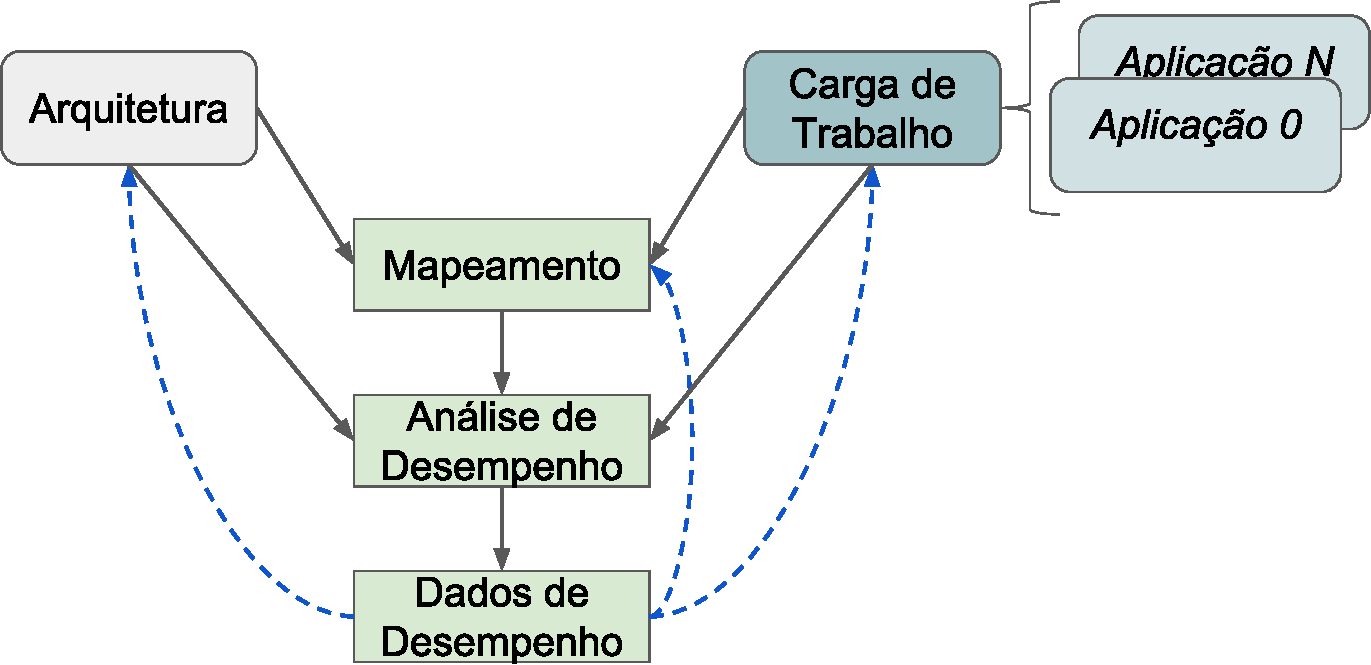
\includegraphics[scale=0.53]{Imagens/y-chart}
	\caption{\label{fig:y-chart} Abordagem \textit{Y-chart} para DSE - adaptado de \cite{gries2004methods}}
\end{figure}

Em resumo, o processo de DSE consiste, a grosso modo, de dois componentes interdependentes \cite{gries2004methods}: (\textit{i}) a avaliação de cada ponto de projeto do espaço de soluções usando, por exemplo, modelos analíticos ou simulação e (\textit{ii}) o mecanismo de busca que sistematicamente percorre o espaço de projeto. Considerando o componente (\textit{i}), o uso de simulação em nível de sistema apresenta características interessantes no que tange aspectos como tempo de simulação e uso de modelos de alto nível (em fases iniciais de desenvolvimento). Quanto ao componente (\textit{ii}), o emprego de heurísticas para a seleção e o direcionamento das buscas por soluções candidatas pode reduzir o tamanho do espaço de projeto (usualmente vasto no caso de projeto de SEs).  


%%%%%%%%%%%%%%%%%%%%%%%%%%%%%%%%%%%%%%%%%%%%%%%%%%%%%%%%
%%%%%%%%%%%     Capítulo ou Seção   %%%%%%%%%%%%%%%%%%%%
%%%%%%%%%%%%%%%%%%%%%%%%%%%%%%%%%%%%%%%%%%%%%%%%%%%%%%%%
\section{Sistemas Heterogêneos de Computação e Aplicações}
%\Topico{Sistemas Heterogêneos. Por que é interessante o aumento da heterogeneidade empregada nos sistemas? Eficiência Energética. Performance.}
Os ambientes de computação atuais estão explorando as capacidades de uma ampla gama de diferentes processadores, tais como CPUs (\textit{central processing units}), processadores de sinais digitais (DSPs - \textit{digital signal processors}), processadores de mídia, processadores vetoriais, hardware reconfigurável (como FPGAs - \textit{Field Programmable Gate Array }) e unidades de processamento gráfico (GPUs - \textit{graphic processing units }) \cite{gaster2012heterogeneous,waidyasooriya2018design}, integrando um relevante número de recursos de processamento heterogêneos e independentes dentro do mesmo sistema \cite{miele2015system}. 

Dado que normalmente as aplicações submetidas aos sistemas apresentam uma série de diferentes comportamentos - desde aplicações intensivas em controle (\textit{control intensive}) - como aplicações de busca, classificação e análise - até aquelas intensas em dados (\textit{data intensive}) - como processamento de imagens, simulação e modelagem, e mineração de dados), não há uma arquitetura única que seja adequada para cada tipo de aplicação \cite{gaster2012heterogeneous}. Além disso, várias partes (trechos) das aplicações podem ser executadas em paralelo (os chamados \textit{kernels} das aplicações), oportunizando a exploração do paralelismo em nível de tarefa (\textit{task-level parallelism} - TLP) \cite{scarpazza2006software}. O TLP pode ser explorado diretamente via sistemas multiprocessados, incluindo aqueles com uma série de PEs heterogêneos.

Computação com recursos heterogêneos, como FPGAs e GPUs, podem melhorar o desempenho e eficiência energética dos sistemas em várias ordens de magnitude. Assim, sistemas heterogêneos surgem com perspectivas de avanço habilitadas, principalmente, pelo abundante paralelismo de dados -- que proporciona a alta capacidade de computação e eficiência energética destes tipos de PEs \cite{rogers2013heterogeneous,durelli2014runtime,waidyasooriya2018design}.



%%%%%%%%%%%%%%%%%%%%%%%%%%%%%%%%%%%%%%%%%%%%%%%%%%%%%%%%
%%%%%%%%%%%     Capítulo ou Seção   %%%%%%%%%%%%%%%%%%%%
%%%%%%%%%%%%%%%%%%%%%%%%%%%%%%%%%%%%%%%%%%%%%%%%%%%%%%%%
\section{Simulação em Nível de Sistema e Modelos de Aplicações e Arquitetura}
%\Topico{Simuladores em nível de ciclo demandam detalhes de implementação. Tempo de simulação proibitivo.}
%\Topico{Simuladores em nível de sistema. Usa modelos de alto nível de abstração. Modelos "Executáveis" de aplicações. Modelos de Arquitetura.}
Simulação é uma forma de avaliar as diferentes soluções para um projeto. Modelagem e simulação usando alto nível de abstração tem um papel importante em fases iniciais de desenvolvimento. Ambas permitem capturar o comportamento do sistema e suas interações, normalmente demandando menores esforços de modelagem (menos detalhes a serem modelados) e de simulação (tempo de simulação) \cite{erbas2007framework}. A utilização de níveis altos de abstração no projeto de SEs é defendida por diversos autores para tratar da complexidade dos projetos \cite{Leite2016}, favorecer abordagens mais rápidas e custo-efetivas que permitam análises relevantes dos complexos espaços de projeto \cite{An2015172}, e que habilitem estimativas no início do projeto baseadas em informações parciais e incertas -- que podem ser utilizadas para guiar o processo de projeto na direção correta \cite{Hendriks2016}. 

Simuladores com precisão de ciclo ou de instrução não podem atender a demanda de processamento necessária em atividades de DSE, dado o alto volume de detalhes sobre o sistema que precisam ser simulados e que podem necessitar de tempos de simulação proibitivos \cite{Herrera201455,gruttner2013complex}. Para contornar os problemas relacionados à simulação com precisão de ciclo tem-se os simuladores em nível de sistema. Segundo Gries \cite{gries2004methods}, durante uma simulação em nível de sistema, a avaliação ocorre em um alto nível de abstração, sendo o sistema representado por uma interconexão de blocos arquiteturais que representam os processadores, as memórias e os barramentos. Assim, modelos de plataforma ou de recursos de processamento (elementos de processamento) representam a arquitetura do sistema \cite{indrusiak2016dynamic}. No caso da  representação da carga de trabalho, as aplicações são descritas por modelos de granulação mais grossa, tais como processos de interação ou mesmo procedimentos inteiros \cite{gries2004methods}. Por exemplo, grafos de tarefas são uma forma comum de representar as cargas de trabalhos (aplicações) no contexto de sistemas embarcados \cite{indrusiak2016dynamic}, sendo esta a forma de representação aplicada em \cite{miele2015system}. Outras formas de representação incluem redes de processo Kahn (KPN - \textit{Kahn Process Networks}) \cite{erbas2007framework}, modelos UML/MARTE \cite{gruttner2013complex,Herrera201455,Leite2016}, modelos de \textit{dataflow} (como \textit{Homogeneous Synchronous DataFlow} - HSDF) \cite{Nogueira2016}, redes de Petri (como \textit{Coloured Petri Net} - CPN) \cite{callou2011energy}, autômatos (como autômatos temporizados - \textit{Timed Automata}) \cite{Jiang:2013:DOM:2491411.2494575,Wang201123}, dentre outros. Estes modelos representam as cargas de trabalho (aplicações) que devem ser submetidas aos sistemas em análise/construção. 

O nível de abstração dos projetos têm sido aumentado para o nível de sistema também com intuito de aumentar a produtividade, gerando um grande interesse em TLM (\textit{Transaction-Level Modeling}) \cite{Cai:2003:TLM}. Com uso de TLM os detalhes sobre comunicação são separados dos componentes de computação por meio do conceito de canais (\textit{channels}). TLM aumenta a velocidade de simulação, permitindo explorar e validar alternativas de projeto em um nível de abstração mais alto \cite{Cai:2003:TLM}. TLM é normalmente utilizada em conjunto com SystemC \cite{patel2008ingredients}. SystemC é  uma linguagem de projeto (\textit{design}) de nível de sistema com forte apoio industrial tendo sido inserida em muitos fluxos de projeto do setor. O uso da infraestrutura do C++ e da sua natureza orientada a objetos estende a usabilidade da SystemC, sendo um meio adequado para a co-simulação de hardware e software \cite{patel2008ingredients}.



%%%%%%%%%%%%%%%%%%%%%%%%%%%%%%%%%%%%%%%%%%%%%%%%%%%%%%%%
%%%%%%%%%%%     Capítulo ou Seção   %%%%%%%%%%%%%%%%%%%%
%%%%%%%%%%%%%%%%%%%%%%%%%%%%%%%%%%%%%%%%%%%%%%%%%%%%%%%%
\section{Abordagens de Exploração do Espaço de Projeto}
%\Topico{O que já foi feito na área (trabalhos relacionados). Problemas/limitações com trabalhos atuais.}

Dada uma determinada carga de trabalho (conjunto de aplicações), os parâmetros de um sistema (referentes a sua arquitetura como, por exemplo, número e tipos de PEs empregados) podem ser devidamente ajustados para encontrar o melhor \textit{trade-off} entre as métricas de sistema avaliadas (por exemplo: energia, área e \textit{delay}). Exploração do Espaço de Projeto (DSE - \textit{Design Space Exploration}) é a ferramenta utilizada para encontrar a \textit{configuração} ótima \cite{Panerati2017}. A tarefa de ajuste dos parâmetros de arquitetura basicamente caracteriza-se como um problema de otimização que envolve a maximização (ou minimização) de múltiplos objetivos --- potencialmente com várias soluções ótimas. A qualidade de uma configuração é expressa pelo conjunto de métricas (ou funções objetivo) utilizadas. O conjunto de soluções ótimas em problemas de otimização multi-objetivos ficam posicionados na chamada \textit{curva de Pareto} --- são os pontos ótimos que não são dominados por nenhum outro ponto \cite{Panerati2017}. 

A obtenção da \textit{curva de Pareto} exige a avaliação de todas as possíveis configurações. No entanto, o vasto tamanho do espaço de projeto é um problema na maior parte dos projetos de sistemas embarcados, e que pode tornar-se ainda mais severo de acordo com os requisitos não-funcionais (restrições) de projeto \cite{Glab2017}. Assim, o principal objetivo da DSE pode ser relaxado no sentido de buscar minimizar o tempo de exploração enquanto garante soluções de boa qualidade \cite{Ascia2011382} (não necessariamente soluções ótimas). Normalmente as abordagens de DSE utilizam estratégias para podar o espaço de projeto e minimizar o número de configurações a serem avaliadas \cite{Ascia2011382}. Heurísticas (ou Meta-Heurísticas) normalmente são aplicadas neste contexto. Meta-heurísticas são metodologias gerais de mais alto nível que podem ser utilizados como estratégias guias no desenvolvimento de heurísticas para solucionar problemas de otimização específicos \cite[p. 1.]{talbi2009metaheuristics}.

Esta seção apresenta algumas abordagens para DSE, incluindo trabalhos elencados em estudo prévio realizado pelo autor desta proposta \cite{Betemps_2017_EQ} (disponível para visualização por meio de link existente no respectivo item na seção de referências), especificamente para o Exame de Qualificação no PPGC da UFPel, no qual foram levantados artigos que tratam sobre o desenvolvimento de Sistemas Embarcados utilizando Alto Nível de Abstração.

Algumas abordagens de DSE utilizam métricas como os artefatos principais no direcionamento da avaliação das soluções candidatas para percorrer o espaço de projeto. Trabalhos como \cite{Gheorghita:2009:SDD:1455229.1455232,Raymond2015,Rodriguez2017,Falkner2016,Altenbernd2016,Hendriks2016,Huang2015} utilizam estimativas relacionadas ao desempenho para o referido propósito. Por outro lado, métricas referentes à Energia consumida ou Potência dissipada são as escolhidas em outras abordagens \cite{Ouni2017203,Jiang:2016:PDT:2872313.2801152,Sorber:2007:ELR:1322263.1322279,Kim_Hong2015}. Métricas relacionadas ao desempenho e energia recorrentemente são utilizadas em abordagens de DSE.
%Hendriks et al. \cite{Hendriks2016} apresentam uma abordagem de engenharia de desempenho de software (\textit{software performance engineering} - SPE), baseada na abordagem \textbf{Y-chart}, focada principalmente em sistemas embarcados intensivos em software. São utilizadas duas diferentes linguagens de modelagem - UPPAAL\footnote{\url{http://www.uppaal.com/}} e JAVA. A abordagem apresenta quatro partes: (i) modelo de aplicação: ressaltando sua estrutura e propriedades; (ii) modelo de execução de tarefas: que trata da dinâmica de execução de tarefas individuais; (iii) modelo de plataforma: descreve os recursos (por exemplo: CPU, RAM) e suas propriedades (como velocidade e capacidade) e algoritmos (que tratam de \textit{scheduling} e alocação); e (iv) modelo de execução de recursos: contém o estado dependente de tempo dos recursos e a dinâmica do recursos (como consumo de energia e DVFS - \textit{dynamic voltage and frequency scaling}).


Em \cite{Falkner2016} é proposta uma abordagem integrada, baseada em modelos abstratos, para a predição de desempenho de sistemas de defesa e sistemas de sistemas (SoS - \textit{Systemsof-Systems}) dirigida por modelo (uma abordagem MDE -- \textit{Model Driven Engineering}). O sistema de prototipação arquitetural utiliza o conceito de cenários e uma série de DSMLs (\textit{domain specific modeling languages}) para a descrição das avaliações a serem realizadas na DSE. Estimativas de tempo em nível de código-fonte são tratadas em \cite{Altenbernd2016} por meio da geração de um Modelo de Tempo a partir do código-fonte (não do executável). Recozimento simulado (\textit{Simulated Annealing}) é utilizado para a obtenção do Modelo Linear de Tempo e, por consequência, o WCET (Tempo Estimado no Pior Caso - \textit{Worst-case Estimation Time}). 

%Em \cite{callou2011energy} é apresentada uma metodologia para avaliação do consumo de energia e tempo de execução em fases iniciais de projeto, sendo que modelos CPN (\textit{Coloured Petri Net} - redes de Petri coloridas) são usados para representar as aplicações.

%Em \cite{Falkner2016} é proposta uma abordagem integrada, baseada em modelos abstratos, para a predição de desempenho de sistemas de defesa e sistemas de sistemas (SoS - \textit{Systemsof-Systems}) dirigida por modelo (uma abordagem MDE -- \textit{Model Driven Engineering}). O sistema de prototipação arquitetural (MEDEA) apresentado suporta uma plataforma experimental dirigida por cenários para avaliar a adequação dos modelos quanto ao conjunto de restrições de desempenho e implantação. MEDEA suporta a modelagem de fragmentos de comportamento dos sistemas constituintes do SoS e de suas interações, alcançados por meio de uma série de DSMLs (\textit{domain specific modeling languages}) que modelam a estrutura e comportamento dos sistemas constituintes, suas interações e as cargas de trabalho que exercitam os modelos em diferentes cenários de desempenho, e as interações entre os sistemas. Estimativas de tempo em nível de Código-fonte são tratadas em \cite{Altenbernd2016} por meio da geração de um Modelo de Tempo a partir do código-fonte (não do executável). Usa execução em hardware nativo ou simulação (simulador \textit{gem5} neste caso) para medir tempo das instruções e faz o mapeamento do código para um conjunto de instruções virtuais (ALF - formato de código para análise estática de programas). Após, usa um emulador (SWEET) para derivar contagem de instruções. Recozimento simulado (\textit{Simulated Annealing}) é utilizado para a obtenção do Modelo Linear de Tempo e, por consequência, o WCET (Tempo Estimado no Pior Caso - \textit{Worst-case Estimation Time}).

O uso de modelos UML \cite{gomaa2011software} e de seus perfis, como MARTE, como elementos centrais de modelagem são aplicados em algumas abordagens de DSE \cite{Herrera201455,gruttner2013complex,Pedre2016}. Uma abordagem de \textbf{Projeto Baseado em Plataforma} para a condução do DSE é utilizada em \cite{gruttner2013complex} como parte de um \textit{framework} de projeto denominado COMPLEX. Modelos UML/MARTE são utilizados para a geração automática de modelos executáveis \textit{SystemC} para fins de validação. A definição do espaço de projeto utiliza o \textit{profile} MARTE onde mapeamentos arquiteturais (espaço de alocação), atributos da plataforma (atributos do espaço) e arquiteturas da plataforma (espaço arquitetural) são definidos. Também associado ao projeto COMPLEX, Herrera et al. \cite{Herrera201455} apresentam uma metodologia para DSE que integra tecnologias de Engenharia Dirigida por Modelos (MDE - \textit{Model Driven Engineering}) e Nível do Sistema Eletrônico (ESL - \textit{Electronic System Level}) juntamente com a exploração de projeto. O espaço de projeto é capturado com o uso de modelos UML/MARTE que permitem a geração de modelos executáveis. A ferramenta de simulação SCoPE+ é utilizada para a avaliação do desempenho das configurações. SCoPE+ inclui uma biblioteca de estimativas de desempenho para diferentes mapeamentos arquiteturais. Uma metodologia de co-projeto (Co-design) para SEs centrados em processador com aceleradores de hardware usando FPGA é apresentada em \cite{Pedre2016}. Orientação a Objetos e UML são utilizados para modelagem das aplicações, C++ para implementação e ferramentas de tradução permitem a tradução semi-automática de código C para HDL.

%O profile UML DIPLODOCUS é utilizado em \cite{Abdallah2016} na abordagem de projeto de SoCs (\textit{System-on-a-Chip}) baseada em MDE para a antecipada exploração do espaço de projeto considerando a dissipação de potência. A abordagem foi implementada no kit de ferramentas \textit{TTool}, na qual conceitos do profile UML DIPLODOCUS e respectivo simulador foram inseridos. Modelos de alto nível são transformados em código funcional de simulação ciente da dissipação de potência visando a tomada de decisões sobre configuração de sistema e técnicas de gerência de potência logo no início do projeto. 

Alguns trabalhos utilizam as capacidades de reconfiguração de dispositivos para lidar com o projeto de SEs. Diguet e seus colegas \cite{Diguet:2011:CSH:1952522.1952531} apresentam um gerenciador de configuração com capacidades de controle e de decisão em tempo de execução para buscar a otimização da arquitetura -- adaptação em tempo de execução. FoRTReSS (\textit{Flow for Reconfigurable archiTectures in Real time SystemS}) \cite{Duhem2015} usa o conceito de Computação Reconfigurável (por intermédio da aplicação de FPGA) para a atividade de alocação de tarefas em elementos de processamento e, possivelmente, utilizando a parte ou região reconfigurável do sistema com intuito de otimização. Aplicações adaptativas em MPSoCs são tratadas em \cite{An2015172}. A DSE é implementada em uma ferramenta protótipo denominada CLASSY (\textit{CLock AnalysiS SYstem}) por meio de busca exaustiva ou por exploração baseada em heurística (algoritmo evolucionário NSGA-II). Em \cite{Huang201088} é apresentada a plataforma de co-projeto de hardware/software baseada em UML (UCoP - \textit{UML-based hardware/software Codesign Platform}). O foco deste trabalho é em sistemas de segurança em rede parcialmente reconfiguráveis dinamicamente (DPRNSS - \textit{Dynamically partially reconfigurable network security systems}) e utiliza a capacidade de reconfiguração de dispositivos FPGA. SEs de segurança crítica são abordados por \cite{Adler:2011:CMV:1880050.1880056}, onde solucionadores de restrições de programação que usam Teoria de Módulo de Satisfação (SMT - \textit{Satisfiability Modulo Theory}) são as ferramentas utilizadas para encontrar configurações preferíveis no espaço de projeto.

\textbf{Algoritmos genéticos} ou, de forma mais geral, \textbf{algoritmos evolucionários}, recorrentemente podem ser observados nas abordagens de DSE apresentadas na literatura. Uma abordagem DSE para Sistemas Embarcados Multimídia é descrita em \cite{Nogueira2016}, no qual as aplicações são representadas como grafos HSDF (\textit{homogeneous synchronous dataflow} - HSDF) e a plataforma de hardware é representada como um grafo dirigido ATG (\textit{Architecture Template Graph}). Um algoritmo genético capaz de lidar com múltiplos objetivos (desempenho, preço e consumo de potência) é utilizado visando encontrar soluções ótimas de Pareto. O formalismo DEVS (técnica formal para modelagem, análise e simulação de sistemas de evento-discreto - \textit{Discrete EVent system Specification}) é utilizado para avaliar as soluções candidatas por meio de simulação. Intervalos de confiança são utilizados como critério de parada das simulações.

Uma abordagem de automação de projeto eletrônico (EDA - \textit{Eletronic Design Automation}) e que aplica algoritmos evolucionários multi-objetivo (MOEA - \textit{Multi-Objective Evolutionary Algorithms}) e técnicas \textit{fuzzy} é apresentada em Ascia et al. \cite{Ascia2011382}. A abordagem de DSE utiliza um aproximador de soluções (sistema \textit{fuzzy}), verificando se a solução obtida é confiável. Quando a solução não é confiável, principalmente durante a fase de treinamento do algoritmo, é utilizada simulação para a geração de métricas. A configuração do sistema é mapeada para uma estrutura de cromossomo e utilizada pelo algoritmo evolucionário em suas interações.
%Um conjunto de soluções de Pareto deve ser obtido como saída do processo de DSE.

Em \cite{Trindade2016}, foram aplicadas diferentes técnicas como programação linear inteira (ILP - \textit{Integer Linear Programming}), algoritmos genéticos (GA) e ferramenta de verificação baseada em SMT (\textit{satisfiability modulo theories}) para resolver um problema de particionamento entre hardware (HW) e software (SW).

Stralen e Pimentel \cite{van2010scenario} utilizam cenários de carga de trabalho (\textit{workloads scenarios}) para capturar o comportamento dinâmico das aplicações (nos níveis intra e interaplicações) e apresenta uma abordagem de DSE baseada em cenário para arquiteturas MPSoCs. A referida abordagem utiliza o conceito de coevolução para avaliar dois problemas simultaneamente: o espaço de projeto do MPSoC e o espaço de cenários para encontrar um subconjunto representativo dos mesmos. Assim, a abordagem usa um algoritmo genético co-evolucionário (\textit{coevolutionary genetic algorithm}).%\Topico{[Problema? Usa traces]. Aplicações como KPN.}

Erbas et al. \cite{erbas2007framework} apresentam o DSE de aplicações multimídia em que as aplicações são representadas por modelos de computação KPN (\textit{Kahn Process Network}) gerados a partir de especificações em C/C++. O ambiente de modelagem e simulação \textit{Sesame} permite a análise de desempenho seguindo os princípios da abordagem \textbf{Y-chart} -- os modelos de arquitetura e aplicações são desacopladas. Para lidar com a otimização multi-objetivos é aplicado o algoritmo evolucionário de Pareto para selecionar soluções ótimas para o mapeamento.

%O problema HAP (\textit{Heterogeneous Assignment with Probability}) é tratado em \cite{Qiu:2009:CMW:1497561.1497568}, onde grafos de fluxo de dados probabilístico (\textit{Probabilistic Data Flow Graph} - PDFG) são usados para descrever as aplicações de um sistema embarcado. Dois algoritmos são apresentados para gerar soluções ótimas e próxima do ótimo descrevendo os melhores elementos de processamento disponíveis na arquitetura para a execução das tarefas das aplicações. O co-projeto de hardware e software também é o foco de trabalhos que tratam da DSE. Uma metodologia de co-projeto (\textit{Co-design}) para sistemas embarcados centrados em processador com aceleradores de hardware usando FPGA é apresentada em \cite{Pedre2016}. Orientação a Objetos e UML são utilizados para modelagem das aplicações, C++ para implementação e ferramentas de tradução permitem a tradução semi-automática de código C para HDL.

De forma geral, os trabalhos se baseiam, direta ou indiretamente, em especificações definidas em nível de código, fazendo com que o nível de abstração utilizado seja menor. Ademais, algumas abordagens exigem conhecimento especializado em linguagens formais específicas, o que ocasiona o aumento de detalhes que necessitam ser modelados e/ou especificados durante as atividades de modelagem.


%%%%%%%%%%%%%%%%%%%%%%%%%%%%%%%%%%%%%%%%%%%%%%%%%%%%%%%%
%%%%%%%%%%%     Capítulo ou Seção   %%%%%%%%%%%%%%%%%%%%
%%%%%%%%%%%%%%%%%%%%%%%%%%%%%%%%%%%%%%%%%%%%%%%%%%%%%%%%
\section{Heurísticas aplicadas na Exploração do Espaço de Projeto}
%O processo de DSE consiste de dois componentes interdependentes \cite{gries2004methods}: (i) a avaliação de um ponto de projeto do espaço de projeto usando, por exemplo, modelos analíticos ou simulação (em nível de sistema) e (ii) o mecanismo de busca que sistematicamente percorre o espaço de projeto. Para o componente (ii) o uso de métodos de otimização ...
%\textbf{(a)} identificação de soluções candidatas plausíveis (i.e., configurações válidas de sistema) e 
%\textbf{(b)} a avaliação de métricas de interesse destas soluções objetivando selecionar configurações ótimas.


Heurísticas, ou Meta-heurísticas, são métodos de solução que controlam a interação entre procedimentos de melhora local e estratégias de alto nível para criar processos capazes de escapar de ótimos locais e que realizem uma busca robusta de um espaço de solução \cite{gendreau2010handbook}. Por outro lado, \cite[p. 1.]{talbi2009metaheuristics} define meta-heurísticas como metodologias gerais de mais alto nível (\textit{templates}) que podem ser utilizados como estratégias guias no desenvolvimento de heurísticas relacionadas para solucionar problemas de otimização específicos .



%%%%%%%%%%%%%%%%%%%%%%%%%%%%%%%%%%%%%%%%%%%%%%%%%%%%%%%%
%%%%%%%%%%%     Capítulo ou Seção   %%%%%%%%%%%%%%%%%%%%
%%%%%%%%%%%%%%%%%%%%%%%%%%%%%%%%%%%%%%%%%%%%%%%%%%%%%%%%
\section{Tema e Contribuições  da Tese}
Nesta Seção são apresentados o \textbf{tema da tese} -- estruturada em três partes: \texttt{Contexto}, \texttt{Questão de Pesquisa} e \texttt{Hipótese} -- e as \textbf{contribuições esperadas} com o desenvolvimento do trabalho em tela.

\subsection{Questão de Pesquisa e Hipótese}

\texttt{Contexto}
\begin{itemize}
\item No contexto de desenvolvimento de sistemas embarcados, sabe-se que o \textit{tamanho do espaço de projeto} pode ser vasto. No caso de um fluxo de projeto de hardware detalhado, a \textit{exploração do espaço de projeto} demanda \textit{proibitivos tempos} para ser realizada de forma completa. \textit{Exploração Precoce do Espaço de Projeto} (\textit{Early DSE}) prevê que, em \textit{fases iniciais} de desenvolvimento, modelos de \textit{alto nível de abstração} para ambos a plataforma e carga de trabalho pretendidas sejam avaliadas, permitindo que o \textit{vasto espaço de projeto} possa ser explorado de forma rápida. Assim, o espaço inicial pode ser reduzido significativamente para ser avaliado de forma detalhada em fluxos tradicionais de projeto de hardware. Considerando o \textit{contexto} descrito, são apresentadas a \textit{Questão de Pesquisa} e \textit{Hipótese} do trabalho.
\end{itemize}

\texttt{Questão de Pesquisa}
\begin{itemize}
\item Considerando o \texttt{contexto} apresentado, como mitigar significativamente o tamanho do espaço de projeto a ser fornecido como entrada em fluxos detalhados de projeto de hardware usando, como base, modelos de alto nível de abstração para a descrição da arquitetura e da carga de trabalho (aplicações) específicas de um sistema, assim como restrições gerais de funcionamento, como energia consumida e desempenho?
\end{itemize}

\texttt{Hipótese}
\begin{itemize}
\item Entende-se que \textit{heurísticas} para seleção de soluções candidatas mais promissoras, sem necessidade da exploração exaustiva de todas as possíveis soluções, possam ser aplicadas em fases iniciais de desenvolvimento com intuito de prover um \textit{espaço de projeto reduzido}. Ademais, \textit{simulação de nível de sistema} pode ser utilizada para gerar dados de avaliação de forma rápida sobre as configurações experimentadas, possibilitando uma análise \textit{comparativa} (ou qualitativa) entre as configurações, mesmo que não forneça dados quantitativamente precisos.
\end{itemize}

\subsection{Contribuições Esperadas da Tese}

\Topico{Diferencial do trabalho em tela? Contribuições?}

\Topico{Uso de heurísticas de seleção de soluções candidatas e simulação em nível de sistema na exploração precoce do espaço de projeto com intuito de minimizar o espaço de projeto a ser explorado em fluxos posteriores mais detalhados quanto ao projeto de hardware}


%Considerando a literatura acadêmica na área de desenvolvimento de sistemas embarcados utilizando alto nível de abstração, observa-se certa tendência em empregar linguagens/modelos semi-formais para representação dos sistemas e suas partes constituintes (módulos, componentes, subsistemas) e do comportamento dinâmico dos mesmos, dado que normalmente são linguagens com menor rigor matemático em sua aplicação e, portanto, que exigem menor expertise por parte dos desenvolvedores para a sua utilização. 



%%%%%%%%%%%%%%%%%%%%%%%%%%%%%%%%%%%%%%%%%%%%%%%%%%%%%%%%
%%%%%%%%%%%     Capítulo ou Seção   %%%%%%%%%%%%%%%%%%%%
%%%%%%%%%%%%%%%%%%%%%%%%%%%%%%%%%%%%%%%%%%%%%%%%%%%%%%%%
\chapter{Objetivos e Resultados}\label{Sec:Objetivos_Resultados}
% (ENTRE 1 e 3 PÁGINAS)
Esta seção apresenta o objetivo geral e objetivos específicos referentes ao doutoramento, assim como os resultados esperados com o desenvolvimento da tese.
%Nesta Seção, apresentam-se o objetivo Geral e os objetivos Específicos da Tese. Os objetivos não devem ser confundidos com as atividades. Para a definição das atividades, deve-se partir dos objetivos determinados nesta Seção. O objetivo Geral do Projeto necessariamente deve ser algum resultado prático (implementação) ou teórico (modelos formais ou especificações ou validações) produto da pesquisa realizada no período do Projeto. Assim como os objetivos específicos, que são considerados como sub-produtos do Objetivo Geral. Além disso, deve-se apresentar os principais resultados esperados do desenvolvimento desta Tese.


%%%%%%%%%%%%%%%%%%%%%%%%%%%%%%%%%%%%%%%%%%%%%%%%%%%%%%%%
%%%%%%%%%%%     Capítulo ou Seção   %%%%%%%%%%%%%%%%%%%%
%%%%%%%%%%%%%%%%%%%%%%%%%%%%%%%%%%%%%%%%%%%%%%%%%%%%%%%%
\section{Objetivo Geral}
%\Topico{Abordar a Exploração do Espaço de Projeto em Fases Iniciais de Desenvolvimento Utilizando Simulação em Nível de Sistema e Modelos em Alto Nível de Abstração Visando o Aumento da Heterogeneidade por meio do Paralelismo em Nível de Tarefa e Considerando Detalhes de Uso de Memória}

\begin{enumerate}[start=0]

\item {Definir e avaliar uma metodologia de \textbf{Exploração Precoce do Espaço de Projeto} (\textit{Early Design Space Exploration - DSE}) usando \textbf{heurísticas} de seleção de soluções candidatas e \textbf{simulação em nível de sistema} na análise de \textit{cargas de trabalho} específicas sobre \textit{arquiteturas multiprocessadas heterogêneas}}.
%\item Propiciar a Exploração do Espaço de Projeto (\textit{Design Space Exploration - DSE}) em Fases Iniciais de Desenvolvimento (\textit{early DSE}) Utilizando Simulação em Nível de Sistema e Modelos em Alto Nível de Abstração Visando o Aumento da Heterogeneidade por meio do Paralelismo em Nível de Tarefa e Considerando Detalhes de Uso de Memória. A Fig. \ref{fig:Contexto_DSE} ilustra o contexto referente ao objetivo geral do trabalho.
\end{enumerate}

A Fig. \ref{fig:FiguraConceitual} ilustra o contexto referente ao objetivo geral do trabalho. Observa-se que o escopo do trabalho engloba a definição da entrada do projeto, consistindo de dados a respeito da carga de trabalho (aplicações), dos elementos da arquitetura do sistema e de restrições associadas ao sistema. Pretende-se que o tamanho do espaço de projeto gerado a partir dos dados de entrada seja reduzido para um conjunto de soluções considerando uma exploração precoce do espaço de projeto utilizando heurísticas de seleção.
%de soluções que proporcione boas soluções e que permita escapar de ótimos locais no decorrer da exploração.
Heurísticas, ou Metaheurísticas, são métodos de solução que controlam a interação entre procedimentos de melhora local e estratégias de alto nível para criar processos capazes de escapar de ótimos locais e que realizem uma busca robusta de um espaço de solução \cite{gendreau2010handbook}.


\begin{figure}[tbp]
\centering
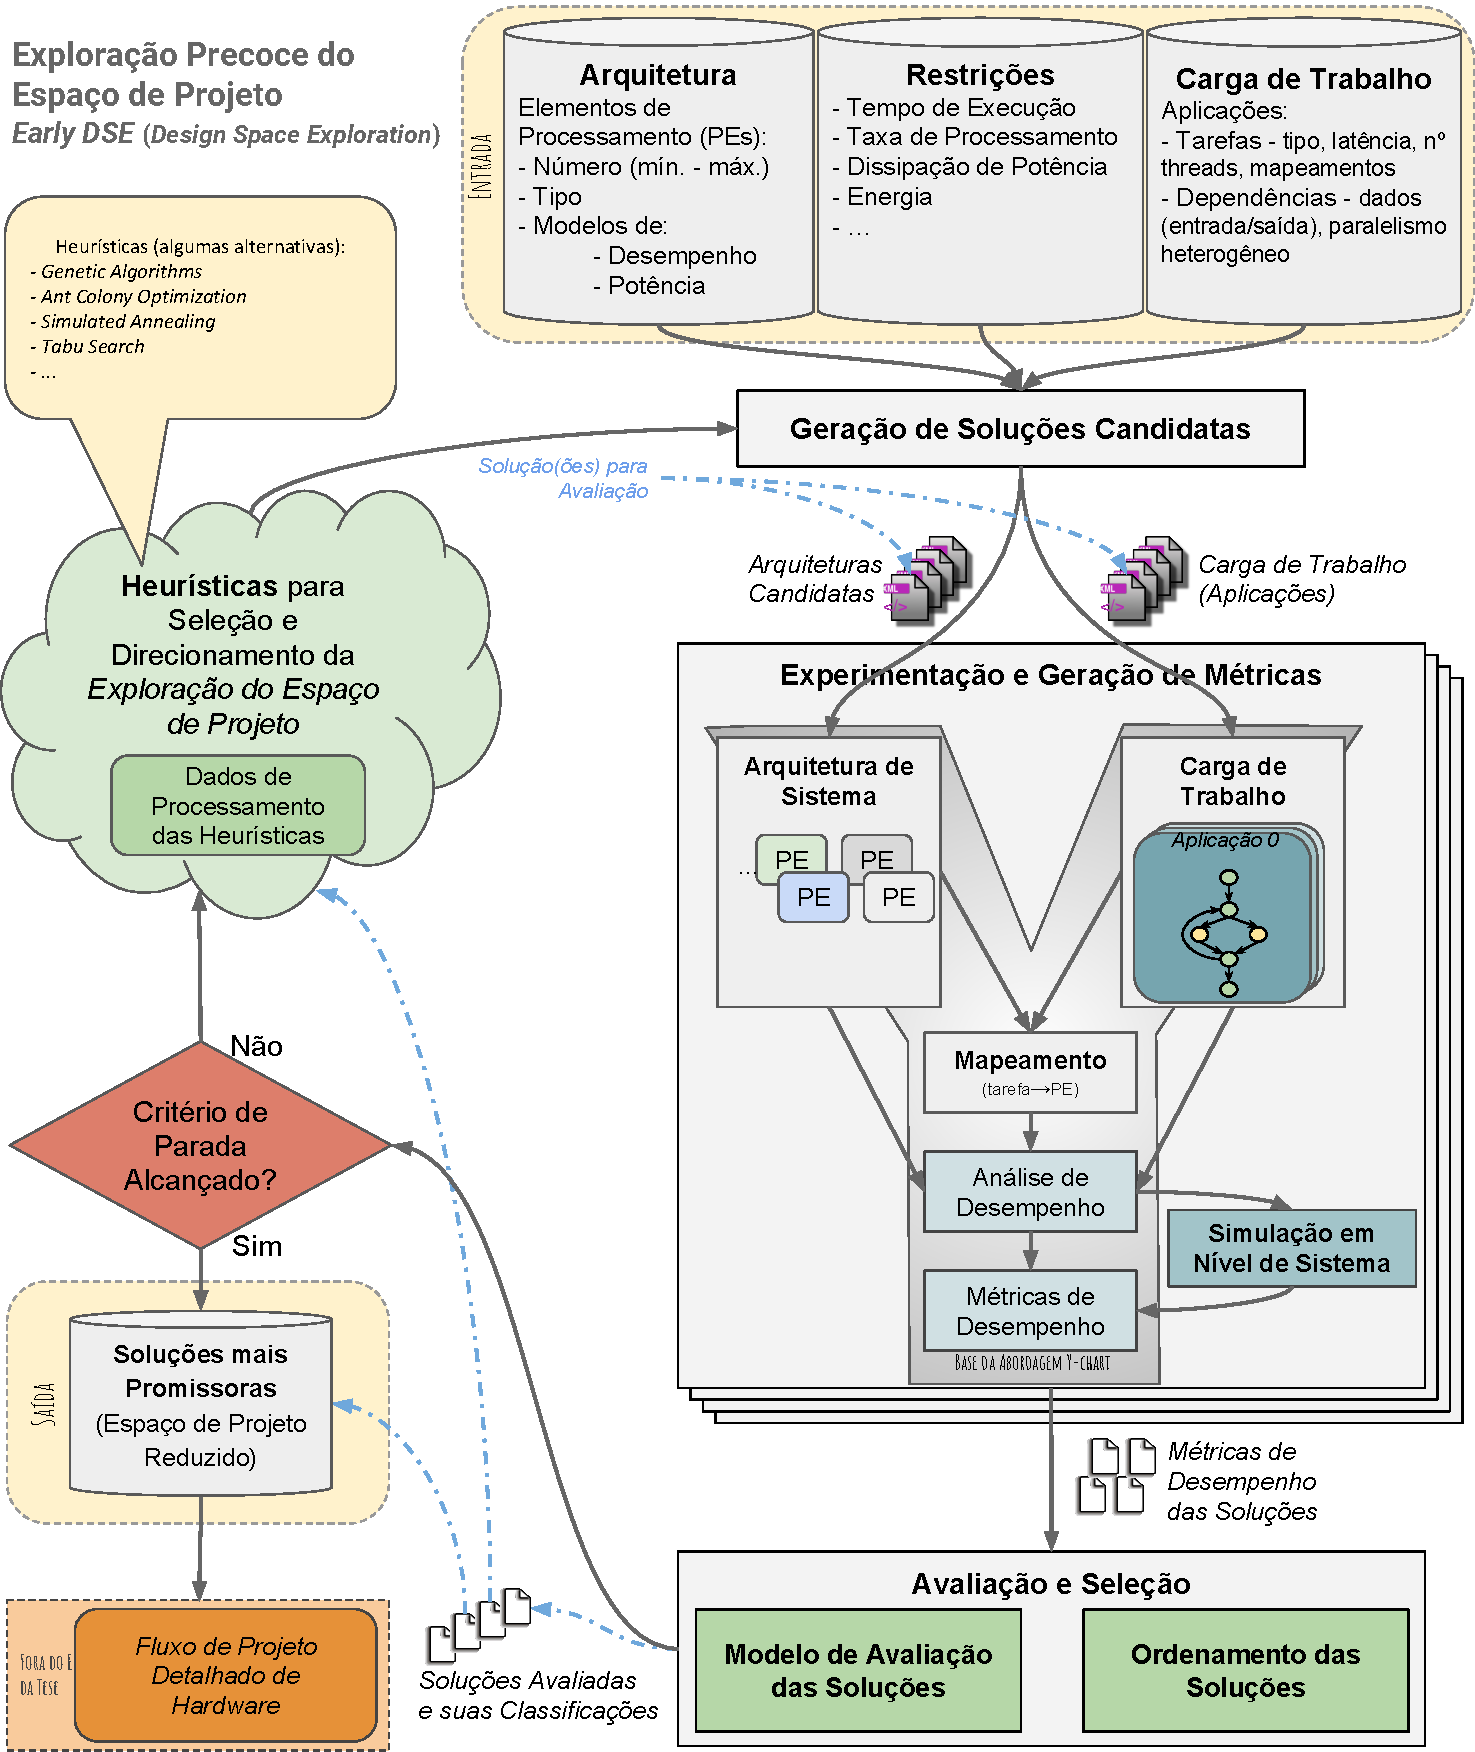
\includegraphics[scale=0.65]{Imagens/Figura_Conceitual_-_Tese}
	\caption{\label{fig:FiguraConceitual} Exploração Precoce do Espaço de Projeto (\textit{Early DSE})}
\end{figure}


%%%%%%%%%%%%%%%%%%%%%%%%%%%%%%%%%%%%%%%%%%%%%%%%%%%%%%%%
%%%%%%%%%%%     Capítulo ou Seção   %%%%%%%%%%%%%%%%%%%%
%%%%%%%%%%%%%%%%%%%%%%%%%%%%%%%%%%%%%%%%%%%%%%%%%%%%%%%%
\section{Objetivos Específicos}
Considerando o \textit{objetivo geral} apresentado, nesta seção são apresentados os \textit{Objetivos Específicos} que detalham cada aspecto necessário ao alcance do objetivo geral:
\begin{enumerate}
\item \textbf{\label{Avaliar o Espaço de Projeto em Fases Iniciais de Desenvolvimento}Avaliar o Espaço de Projeto em Fases Iniciais de Desenvolvimento}: em fases iniciais de desenvolvimento pode não estar disponível a arquitetura de sistema ou mesmo as aplicações para a realização de testes. Assim, modelos em alto nível de abstração e simulação em nível de sistema podem ser aplicados para a realização da Exploração do Espaço de Projeto em fases iniciais de desenvolvimento (em inglês: \textit{Early Design Space Exploration}), permitindo a tomada de decisões mesmo em situações onde não há disponibilidade de aplicações ou mesmo arquitetura de sistema para a realização de experimentos.
\item \textbf{\label{Empregar Heurísticas na Seleção de Soluções Candidatas}Empregar Heurísticas na Seleção de Soluções Candidatas}: avaliar a utilização de diferentes heurísticas para otimizar o processo de seleção de soluções candidatas. Algumas alternativas são Algoritmos Genéticos (GA - \textit{Genetic Algorithms})\cite{Reeves2010_GA}, recozimento simulado (\textit{Simulated Annealing}) \cite{Nikolaev2010_Simul_Anneal}, Busca Tabu (\textit{Tabu Search}) \cite{Gendreau2010_Tabu}  e Otimização de Colonia de Formigas (ACO - \textit{Ant Colony Optimization}) \cite{Dorigo2010_ACO}, dentre outras alternativas passíveis de avaliação.
\item \textbf{\label{Utilizar Simulação em Nível de Sistema}Utilizar Simulação em Nível de Sistema}: modelos de granularidade mais alta são utilizados em simuladores de nível de sistema. Estes simuladores normalmente permitem a rápida simulação de possíveis soluções de um dado projeto; além de utilizarem modelos de aplicações e de arquitetura normalmente gerados com menor esforço de modelagem.
\item \textbf{\label{Empregar Modelos de Alto Nível de Abstração no DSE}Empregar Modelos de Alto Nível de Abstração no DSE}: modelos de alto nível são usados para descrever \textbf{aplicações} e \textbf{arquitetura} do sistema (basicamente, seus elementos de processamento) visando a rápida geração destes modelos para avaliação em fases iniciais de desenvolvimento. %Além disso, considerar aspectos de funcionamento da \textbf{memória} de sistema (como transferências e contenção) a partir da caracterização dos dados de entrada e saída das tarefas (\textit{task}) modeladas nas aplicações.
\item \textbf{\label{Aproveitar a Heterogeneidade de Processamento Existente na Arquitetura dos Sistemas}Aproveitar a Heterogeneidade de Processamento Existente na Arquitetura dos Sistemas}: considerar as diferentes características dos \textit{kernels} das aplicações e aproveitá-las na alocação dos heterogêneos elementos de processamento (PE) existentes no sistema. Os \textit{kernels} de aplicação podem ser executados em diferentes tipos de PE, até mesmo por mais de um simultaneamente, e utilizando uma ou mais \textit{threads} de execução. Propiciar que possam ser utilizados como elementos de processamento pelos menos CPUs, GPUs e FPGAs. Outros elementos como DSPs (\textit{Digital Signal Processor}), ASICs (\textit{Application-Specific Integrated Circuit}) e ASIPs (\textit{Application-Specific Instruction-set Processor}) também podem ser avaliados no contexto do trabalho.

%\item \Topico{Particionamento dos dados de entrada de uma tarefa e os tipos de unidades de processamento disponíveis na alocação de recursos?? Considerando que os diferentes PE possuem suas próprias estruturas de memória, e que a transferência de dados entre a memória principal e a memória de cada dispositivo dos PEs podem ser feitas em paralelo, será possível minimizar (ou ocultar) a latência da transferência de dados entre as memórias? O particionamento dos dados a serem processados pode ser feito considerando a latência das transferências entre memórias e a latência dos próprios PEs? Qual a sobrecarga de acesso paralelo à memória principal? A mesma suporta? HMC (\textit{Hybrid Memory Cube}) se encaixa nesta situação? Região de Memória onde é feita a carga do programa e seus dados pode influenciar na latência de acesso (em paralelo) aos dados das diferentes aplicações em execução simultânea}

\end{enumerate}


%%%%%%%%%%%%%%%%%%%%%%%%%%%%%%%%%%%%%%%%%%%%%%%%%%%%%%%%
%%%%%%%%%%%     Capítulo ou Seção   %%%%%%%%%%%%%%%%%%%%
%%%%%%%%%%%%%%%%%%%%%%%%%%%%%%%%%%%%%%%%%%%%%%%%%%%%%%%%
\section{Resultados Esperados}
%\Topico{Resultados Esperados??? Metodologia de DSE? Algoritmo de Alocação de Recursos? }
Como principal resultado esperado do desenvolvimento do trabalho pode-se indicar a definição de uma \textbf{Metodologia de Exploração Precoce do Espaço de Projeto} (\textit{Early DSE} - \textit{Design Space Exploration}) a ser aplicada em \textit{fases iniciais} de projetos de desenvolvimento de \textit{Sistemas Embarcados}, considerando \textit{restrições} gerais de projeto e \textit{modelos} em alto nível de \textit{abstração} para as aplicações e arquitetura do sistema, também buscando ampliar a \textit{heterogeneidade} aplicada na execução da carga de trabalho (\textit{workload} - aplicações) submetida para tirar proveito das diferentes características das \textit{tasks} (especificamente os \textit{kernels}) constituintes de cada aplicação.
%e aspectos de utilização da \textit{memória} do sistema.



%%%%%%%%%%%%%%%%%%%%%%%%%%%%%%%%%%%%%%%%%%%%%%%%%%%%%%%%
%%%%%%%%%%%     Capítulo ou Seção   %%%%%%%%%%%%%%%%%%%%
%%%%%%%%%%%%%%%%%%%%%%%%%%%%%%%%%%%%%%%%%%%%%%%%%%%%%%%%
\chapter{Metodologia}\label{sec:Metodologia}

% (ENTRE 1 e 3 PÁGINAS)
%Nesta Seção, apresenta-se a metodologia proposta para o desenvolvimento da Tese. O proponente deve descrever as atividades necessárias para a conclusão dos objetivos propostos.
Esta Seção apresenta a metodologia de trabalho para o desenvolvimento e alcance dos objetivos geral e específicos previamente apresentados. Inicialmente são apresentadas as atividades previstas, seguidas pela apresentação do ferramental e subsídios necessários ao andamento do trabalho.


%%%%%%%%%%%%%%%%%%%%%%%%%%%%%%%%%%%%%%%%%%%%%%%%%%%%%%%%
%%%%%%%%%%%     Capítulo ou Seção   %%%%%%%%%%%%%%%%%%%%
%%%%%%%%%%%%%%%%%%%%%%%%%%%%%%%%%%%%%%%%%%%%%%%%%%%%%%%%
\section{Atividades para o Desenvolvimento do Trabalho}
Para o alcance dos objetivos geral e específicos apresentados na Seção \ref{Sec:Objetivos_Resultados}, o seguinte conjunto de atividades precisa ser executado para contemplar cada um dos objetivos específicos do trabalho que, por sua vez, propiciam o alcance do Objetivo Geral do Trabalho. 

\begin{enumerate}[start=0]
\item(Objetivo Geral) Definir e avaliar uma metodologia de \textbf{Exploração Precoce do Espaço de Projeto} (\textit{Early Design Space Exploration - DSE}) usando \textbf{heurísticas} de seleção de soluções candidatas e \textbf{simulação em nível de sistema} na análise de \textit{cargas de trabalho} específicas sobre \textit{arquiteturas multiprocessadas heterogêneas} 

 \begin{enumerate}
     \item \Topico{Escrever, Revisar e Entregar Texto da Tese de Doutorado}
     \item \Topico{Preparar e Realizar a Defesa da Tese de Doutorado}
 \end{enumerate}
\item(Objetivo) {Avaliar o Espaço de Projeto em Fases Iniciais de Desenvolvimento}
\begin{enumerate}
\item Estruturar o ambiente necessário para Exploração do Espaço de Projeto em fases iniciais de desenvolvimento;
\item Avaliar e definir métricas que possam ser utilizadas para avaliação de desempenho;
\item Avaliar e definir o formato e estrutura dos dados de entrada do DSE, considerando aspectos de(a):
	\begin{itemize}
    	\item \underline{Arquitetura do sistema}: número e tipo de elementos de processamento; modelos de potência e de desempenho;
        \item \underline{Carga de trabalho a ser submetida ao sistema}: descrição das aplicações e suas tarefas (\textit{tasks});
        \item \underline{Restrições de Projeto referentes ao sistema ou aplicações}, como, por exemplo: tempo de execução, taxa de processamento (\textit{throughput}), dissipação de potência, consumo de energia, dentre outros possíveis.
    \end{itemize}
\item Elencar, avaliar e definir \textit{estratégias de geração de soluções candidatas} que possam ser utilizadas considerando os dados de entrada;
\item Elencar, avaliar e definir modelo(s) de avaliação da qualidade das soluções (configurações) experimentadas na Exploração Precoce do Espaço de Projeto;
\item Estruturar e documentar a metodologia definida para \textit{Early DSE};
\item Projetar experimento de avaliação da metodologia de \textit{Early DSE}.
\end{enumerate}

\item(Objetivo) {Empregar Heurísticas na Seleção de Soluções Candidatas}
\begin{enumerate}
\item Buscar, na literatura acadêmica, por heurísticas de seleção de soluções candidatas a serem aplicadas em uma metodologia de DSE;
\item Avaliar e elencar as heurísticas (inicialmente pretende-se utilizar quatro heurísticas: \textbf{A}--\textbf{D}) encontradas na literatura;
\item Projetar, Implementar e Conduzir experimento de avaliação da heurística \textbf{A};
\item Projetar, Implementar e Conduzir experimento de avaliação da heurística \textbf{B};
\item Projetar, Implementar e Conduzir experimento de avaliação da heurística \textbf{C};
\item Projetar, Implementar e Conduzir experimento de avaliação da heurística \textbf{D}.
\end{enumerate}

\item(Objetivo) {Utilizar Simulação em Nível de Sistema}
\begin{enumerate}
\item Avaliar e definir simulador que possa ser utilizado na rápida simulação de uma dada carga de trabalho executada sobre uma arquitetura de sistema. O simulador SAVE \cite{miele2015system} apresenta características promissoras para a implementação e teste das hipóteses a serem trabalhadas na tese. O referido simulador foi alterado para permitir a execução em paralelo, e para a mesma aplicação, de tarefas (\textit{tasks}) implementadas para diferentes elementos de processamento (como CPU e GPU). O simulador com estas alterações passou a ser denominado \texttt{SAVE-htlp} (onde \texttt{htlp} significa \textit{heterogeneous task-level parallelism}). A Seção \ref{SAVE_htlp} descreve superficialmente o referido simulador;
\item Implementar e adicionar ao simulador \texttt{SAVE-htlp} uma unidade de processamento que se enquadre como Reconfigurável, do tipo FPGA (\textit{Field Programmable Gate Array} - Matriz de Portas Programáveis em Campo) ou CGRA (\textit{Coarse Grained Reconfigurable Architecture} - Arquitetura Reconfigurável de Grossa Granulação) \cite{Mansureh2017}.

\end{enumerate}

\item(Objetivo) {Empregar Modelos de Alto Nível de Abstração no DSE}
\begin{enumerate}
\item Avaliar e definir modelos em alto nível de abstração que possam ser utilizados como entrada de projeto para o detalhamento de carga de trabalho (aplicações), arquitetura do sistema (elementos de processamento), e alternativas de mapeamento dos \textit{kernels} das aplicações. A seção \ref{SAVE_htlp} descreve alguns aspectos do simulador SAVE-htlp, incluindo os modelos de arquitetura e aplicações (\textit{workload}) utilizados pelo referido simulador, os quais julga-se adequados para utilização no contexto deste trabalho;
\item Estudar formas automatizadas ou semi-automatizadas para a geração de modelos de arquitetura e de carga de trabalho de um sistema em avaliação, assim como as alternativas de mapeamento disponíveis.
\end{enumerate}

\item(Objetivo) {Aproveitar a Heterogeneidade de Processamento Existente na Arquitetura dos Sistemas}
\begin{enumerate}
\item Garantir a geração de soluções candidatas que considerem a utilização de todas as diferentes unidades de processamento existentes na arquitetura do sistema;
\item Garantir a geração de soluções candidatas que considerem, quando possível, a utilização simultânea de unidades de processamento heterogêneas para a execução de tarefas (especificamente \textit{kernels} de aplicações) de mesmo objetivo (porém com implementações para diferentes tipos de elementos de processamento). No contexto deste trabalho esta possibilidade é denominada de Paralelismo Heterogêneo em Nível de Tarefa - HLTP (\textit{Heterogeneous Task-level Paralelism}).
\end{enumerate}

\end{enumerate}	


%%%%%%%%%%%%%%%%%%%%%%%%%%%%%%%%%%%%%%%%%%%%%%%%%%%%%%%%
%%%%%%%%%%%     Capítulo ou Seção   %%%%%%%%%%%%%%%%%%%%
%%%%%%%%%%%%%%%%%%%%%%%%%%%%%%%%%%%%%%%%%%%%%%%%%%%%%%%%
\section{Obrigações Regimentais junto ao PPGC/UFPel}
Considerando o regimento do Programa de Pós-Graduação em Computação da Universidade Federal de Pelotas, nesta seção são abordadas as atividades obrigatórias referentes ao curso de Doutorado. As atividades obrigatórias do programa são descritas abaixo, seguidas por um breve histórico da respectiva atividade ou uma descrição sobre o planejamento para a execução da mesma.

% 	\item \Topico{Cursar os Créditos Obrigatórios\footnote{\label{Obr_PPGC_}Obrigações regimentais junto ao PPGC/UFPel} do PPGC UFPel}
%     \item \Topico{Preparar e Apresentar o Exame de Qualificação\footnoteref{Obr_PPGC}} 
%     \item \Topico{Preparar e Defender a Proposta de Tese\footnoteref{Obr_PPGC}}
%     \item \Topico{Preparar e Apresentar Seminário de Andamento\footnoteref{Obr_PPGC}}
%     \item \Topico{Escrever e Submeter Artigo(s) em Evento/Periódico da Área de Interesse}
\begin{enumerate} %obrigações regimentais junto ao PPGC/UFPel
	\item \Topico{Cursar os Créditos Obrigatórios do programa}: atualmente (2018/1) 38 créditos já foram aproveitados ou cursados em disciplinas ofertadas pelo PPGC/UFPel;
    \item \Topico{Preparar e Apresentar o Exame de Qualificação}: em Outubro de 2017 foi apresentado o Exame de Qualificação junto a banca de avaliação, sendo considerado Aprovado;
    \item \Topico{Preparar e Defender a Proposta de Tese}: atividade que gerou a proposta em tela e que deve ser ser defendida (até o prazo máximo de 15 de Outubro de 2018) perante arguição de banca específica para este fim;
    \item \Topico{Preparar e Apresentar Seminário de Andamento}: até o final do semestre 2018/2 deverá ser apresentado o Seminário de Andamento. Este tem por finalidade apresentar as atividades desenvolvidas no trabalho considerando a proposta previamente avaliada;
    \item \Topico{Escrever e Submeter Artigo(s) em Evento/Periódico da Área de Interesse}: o regimento do PPGC/UFPel aponta como necessária a submissão e publicação de artigo(s) que descrevem resultados do trabalho desenvolvido durante o doutoramento.
    \item \Topico{Escrever, Revisar e Entregar Texto da Tese de Doutorado}
    \item \Topico{Preparar e Realizar a Defesa da Tese de Doutorado}
\end{enumerate}



%%%%%%%%%%%%%%%%%%%%%%%%%%%%%%%%%%%%%%%%%%%%%%%%%%%%%%%%
%%%%%%%%%%%     Capítulo ou Seção   %%%%%%%%%%%%%%%%%%%%
%%%%%%%%%%%%%%%%%%%%%%%%%%%%%%%%%%%%%%%%%%%%%%%%%%%%%%%%
\section{Subsídios e Ferramentas para o Desenvolvimento do Trabalho}
De forma geral, o levantamento de referências da literatura acadêmica será realizado com base em bibliotecas digitais (ou repositórios) e ferramentas de busca especializadas disponíveis na internet. Também poderão ser consultados títulos disponíveis nas bibliotecas da instituição. Algumas bibliotecas digitais e fontes de consulta que podem ser utilizadas são:
\begin{itemize}
\item IEEEXplore - \url{https://ieeexplore.ieee.org/Xplore/home.jsp};
\item ACM Digital Library - \url{https://dl.acm.org/};
\item Elsevier - Science Direct - \url{https://www.sciencedirect.com/};
\item Springer Link - \url{https://link.springer.com/};
\item Google Acadêmico - \url{https://scholar.google.com.br/};
\end{itemize}

Com respeito aos equipamentos necessários para o desenvolvimento do trabalho, dado que não há necessidade, \textit{a priori}, de equipamentos especiais para a condução do trabalho, serão utilizados computadores/servidores disponíveis nos laboratórios da instituição, assim como \textit{notebook} pessoal do autor do trabalho. Nos referidos computadores/servidores poderão ser realizadas tarefas gerais relacionadas às atividades de modelagem, escrita, simulação, programação, revisão, projeto e definição de experimentos, tratamento e organização de dados, edição e geração de gráficos e figuras, dentre outras que forem julgadas necessárias ao trabalho.


\subsection{SAVE-htlp - Simulador em Nível de Sistema}\label{SAVE_htlp} 
Em \cite{miele2015system} é apresentado um simulador implementado em SystemC e TLM para validar políticas de gerência de recursos em Arquiteturas de Sistemas Heterogêneos (\textit{Heterogeneous System Architectures} - HSA) \cite{HSA_Foundation}. O simulador \cite{miele2015system} busca lidar com gerenciamento em tempo de execução na alocação de recursos de processamento para as aplicações, baseado na eficiência das unidades de processamento e para atender requisitos de nível de serviços (na forma de um \textit{Service Level Agreement}). As aplicações são modeladas como grafos de tarefas que incluem informações sobre os tipos de tarefas e suas latências, contadores de desempenho, números de linhas de execução (\textit{threads}), dentre outros. A arquitetura de hardware é modelada como um conjunto de recursos genéricos que descrevem modelos de desempenho e de potência. A Fig. \ref{fig:Sim_Input} ilustra modelos de aplicação e de arquitetura utilizados no referido simulador. A parte de Software (SW) da plataforma virtual é descrita à esquerda da figura. Cada nó do grafo representa uma tarefa (\textit{task}) da aplicação, sendo caracterizadas pela latência de execução em algum modelo de elemento de processamento (PE), frequência de operação, tipo de tarefa (\textit{elaboration} ou \textit{main}), tamanho dos dados de entrada e saída e, quando for o caso, ponto de chamada da função de atualização de \textit{heartbeats} \cite{Hoffmann:2010}. Além disso, para cada tarefa são definidos os mapeamentos possíveis para as unidades de processamento existentes. A arestas representam as dependências entre as tarefas e são caracterizadas pelo seu tipo e número de ciclos (para este último o valor \textit{default} é 1). Os aspectos da arquitetura (Hardware - HW) são descritos no lado direito da figura. Os elementos de processamento da arquitetura são descritos pelo seu tipo, modelo, e dados de \textit{dvfs} (\textit{dynamic voltage and frequency scaling}). Os dados de \textit{dvfs} são frequência de operação, potência em operação (\textit{Power}) e potência em estado ocioso (\textit{IdlePower}). Pelo menos uma descrição de \textit{dvfs} deve existir para cada unidade de processamento.


\begin{figure}[t]
\centering
		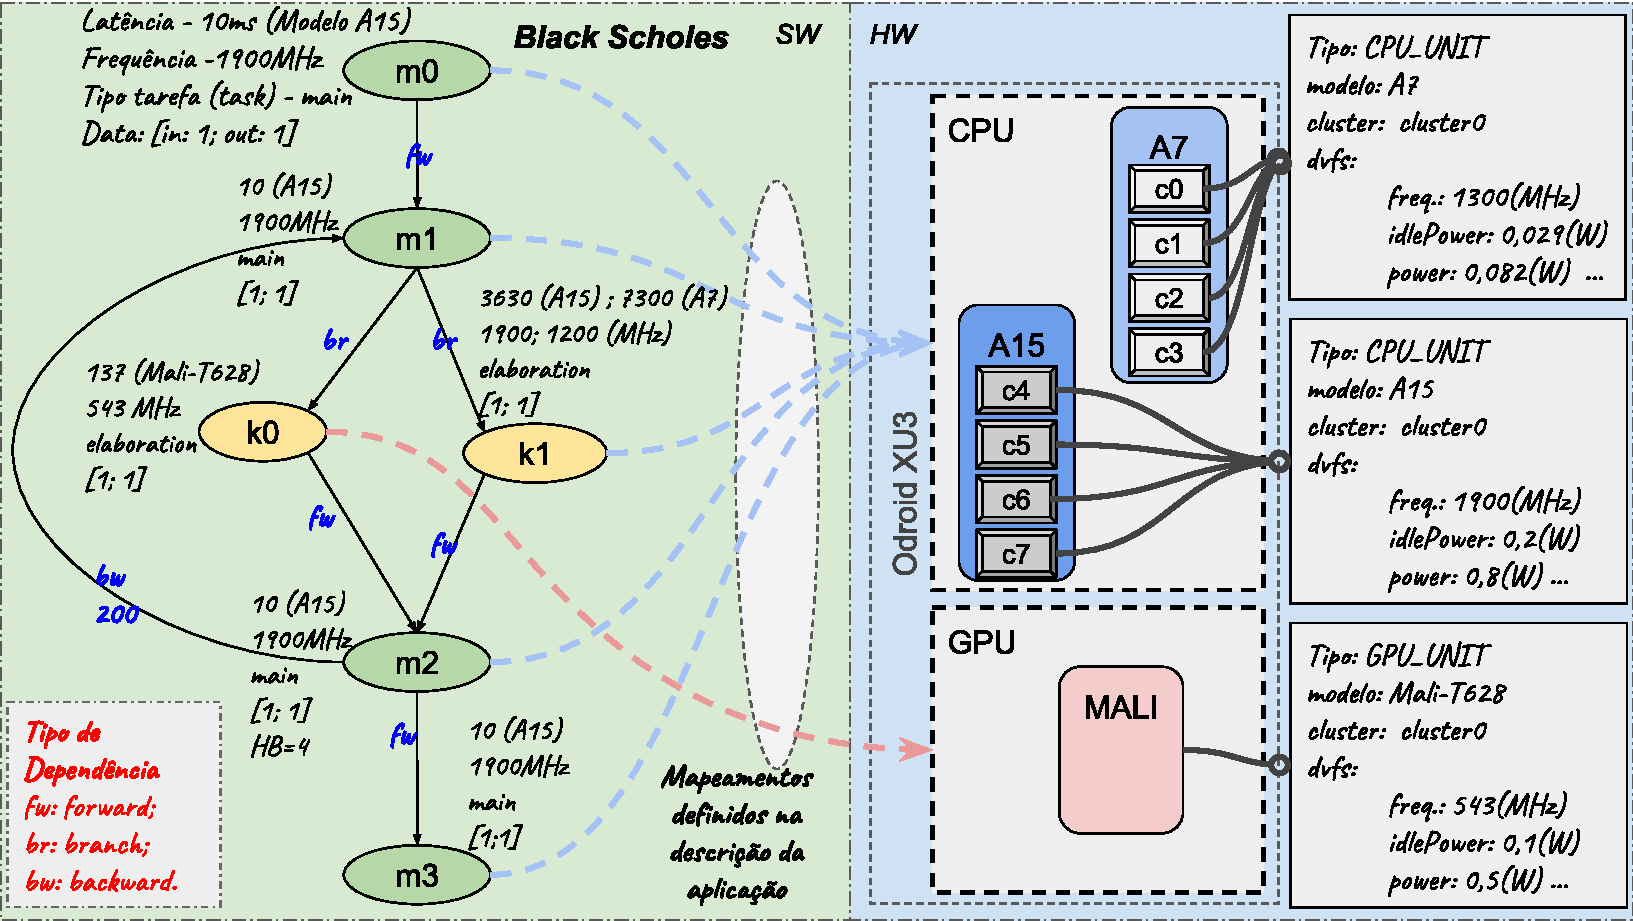
\includegraphics[scale=0.58]{Imagens/Sim_Input}
	\caption{\label{fig:Sim_Input} Modelos de Aplicação e Arquitetura no Simulador \textit{SAVE-htlp}}
\end{figure}

Foi obtido junto aos autores do referido simulador \cite{miele2015system} acesso ao respectivo código-fonte e este parece promissor quanto às possibilidades de extensão que possam ser incorporadas como parte do trabalho de doutorado para implementação, testes e avaliação das hipóteses da tese. Assim, este simulador foi adaptado visando o aumento da heterogeneidade aplicada na execução de aplicações que possuam \textit{tasks} (\textit{kernels}) com paralelismo em nível de tarefa (TLP) e que permitam a criação e execução simultânea de \textit{threads} destinadas à distintas unidades de processamento (tais como CPUs e GPUs). A versão modificada no simulador passou a ser denominada SAVE-htlp (onde \textit{htlp} significa \textit{heterogeneous task-level parallelism} - paralelismo heterogêneo em nível de tarefa). Com o SAVE-htlp foram planejados e realizados alguns experimentos usando diferentes configurações para a arquitetura do sistema, combinando as \textit{threads} referentes às \textit{tasks} das aplicações com diferentes unidades de processamento e variando o número de \textit{threads} executadas em cada caso. Nos experimentos, um modelo de arquitetura baseado na plataforma ODROID XU3 \cite{HardKernel_Odroid_XU3} foi empregado e, como estudo de caso, foi utilizada uma aplicação de \textit{Block Matching Algorithm} (BMA - Algoritmo de Correspondência de Blocos). BMA é aplicado em áreas como codificação de vídeo e visão computacional e para os experimentos foi utilizada como base as implementações apresentadas por Melo et al. \cite{melo2016parallel}. Considerando os resultados dos experimentos foi escrito um artigo científico, com o título “\textit{Exploring Heterogeneous Task-Level Parallelism in a BMA Video Coding Application using System Level Simulation}”, e submetido ao evento SBESC 2018\footnote{\url{http://sbesc.lisha.ufsc.br/sbesc2018/Home}} - atualmente o artigo está em processo de análise pelo comitê de programa do evento.
%com o título “\textit{Exploring Heterogeneous Task-Level Parallelism using System-Level Simulation}”, e submetido ao evento SBCCI 2018\footnote{\url{https://wp.ufpel.edu.br/chipinthepampa2018/events/sbcci-2018/}} - não sendo aceito para publicação no referido evento. Uma versão revisada do artigo está em preparação para submissão ao SBESC 2018\footnote{\url{http://sbesc.lisha.ufsc.br/sbesc2018/Home}}.



%%%%%%%%%%%%%%%%%%%%%%%%%%%%%%%%%%%%%%%%%%%%%%%%%%%%%%%%
%%%%%%%%%%%     Capítulo ou Seção   %%%%%%%%%%%%%%%%%%%%
%%%%%%%%%%%%%%%%%%%%%%%%%%%%%%%%%%%%%%%%%%%%%%%%%%%%%%%%
\chapter{Cronograma}
%Esta Seção deve apresentar relação numerada de atividades (de estudo, modelagem, especificação, implementação ou validação) que deverão ser realizadas e o cronograma destas atividades.
Esta seção apresenta o cronograma de realização das atividades necessárias para o alcance do objetivo geral do trabalho. As atividades estão descritas na Seção \ref{sec:Metodologia}, tendo sido descritas e identificadas conforme o objetivo específico ao qual cada atividade está mais diretamente relacionada.

\Topico{Inserir diagrama de Gannt relacionando as atividades, suas dependências e respectivos prazos }



\chapter{Anotações}

\section {Referência: \cite{Panerati2017}}

Abordagens de DSE normalmente necessitam utilizar simulação (ou estimativa) para avaliar as métricas no nível do sistema (ou seja, as funções objetivo) do grande número de configurações que são examinadas.

A automação de DSE envolve dois sub-problemas: 
\begin{itemize}
\item \textbf{(a)} identificação de soluções candidatas plausíveis (i.e., configurações válidas de sistema) e 
\item \textbf{(b)} a avaliação de métricas de interesse destas soluções objetivando selecionar configurações ótimas.
\end{itemize}

Algoritmos Evolucionários (EAs - \textit{Evolutionary Algorithms}) são amplamente usados em DSE. EAs discriminam e selecionam soluções usando uma combinação de métricas representadas por uma função de \textit{fitness}. Além disso, EAs são normalmente fáceis de aplicar e não necessitam conhecimento detalhado do espaço a ser explorado.
Abordagens Evolucionárias para otimização multi-objetivos (classificação): 
\begin{enumerate}
\item Algoritmos que utilizam funções agregadoras (\textit{aggregating functions})
\item Algoritmos que utilizam funções não-agregadoras (\textit{non-aggregating functions}) mas abordagens não baseadas em Pareto
\item Abordagens baseadas em Pareto
\end{enumerate}

Considerando um escopo mais amplo, para além das abordagens evolucionárias, classificam-se as abordagens para o sub-problema (a) em:
\begin{itemize}
\item \textbf{Classe 1}: \textit{Abordagens de Otimização Pseudo Aleatória e Heurísticas}. Estas abordagens normalmente trabalham com a ideia de \textit{clusters} a serem explorados exaustivamente. Exemplos: Otimização por multi-agentes (como \textit{Particle Swarm Optimization} - PSO), Recozimento Simulado (\textit{Simulated Annealing} - SA), Busca Tabu (\textit{Tabu Search}) e Algoritmos de Pesquisa de Operações (\textit{operations research algorithms});
\item \textbf{Classe 2}: \textit{Algoritmos Evolucionários}. Caracterizam-se por modificações aleatórias sobre o conjunto inicial de configurações buscando de forma iterativa melhorar o conjunto de soluções de Pareto. Exemplos: Algoritmos Genéticos (\textit{Genetic Algorithms} - GA). Técnicas podem ser combinadas com métodos exatos - e.g.: DSE é transformado em um problema de Programação Linear Inteira 0-1 Multi-Objetivos e um solucionador pseudo-Booleano (PB) é usado para restringir o GA dentro de um espaço de busca factível.
\item \textbf{Classe 3}: \textit{Abordagens Estatísticas sem Conhecimento do Domínio}. Usam um \textit{metamodelo} extraído do domínio para prever as próximas configurações a serem avaliadas - e.g.: Projeto de Experimentos (\textit{Design of Experiments} - DoE).
\item \textbf{Classe 4}: \textit{Abordagens Estatísticas com Conhecimento do Domínio}. Utilizam regras pré-definidas e conhecimento específico do espaço de projeto para encontrar as soluções mais promissoras. É criado um  framework probabilístico para guiar a identificação de novas soluçõe candidatas. E.g.: Processo de Decisão de Markov (\textit{Markov Decision Process} - MDP).
\end{itemize}

Para o sub-problema \textbf{(b)} a DSE pode ser conduzida por meio de \textbf{simulação detalhada} ou \textbf{modelos preditivos mais simples}, ou mesmo uma combinação de ambos.

Exemplos de algumas Métricas para Avaliação de Conjuntos Aproximados de Pareto:

- (a) ADRS - \textit{Average Distance from Reference Set}

- (b) \textit{Non-uniformity}

- (c) \textit{Concentration}


Esforços Iniciais de Configuração e Sensitividade dos Parâmetros (\textit{Initial Setup Effort and Parameter Sensitivity})

Exemplos de \textit{frameworks} e bibliotecas para Problemas de Otimização Multi-Objetivos: jMetal (\url{http://jmetal.sourceforge.net/}), PaGMO/PyGMO (\url{https://github.com/esa/pagmo/} --> \url{https://github.com/esa/pagmo2}), MOMHLib++ (\url{https://github.com/derino/maponoc/tree/master/libs/libmomh-1.91.3}) e NASA (\textit{Non Ad-hoc Search Algorithm}).







\begin{comment}
\begin{table}[ht]
\centering
\caption{Resumo das Atividades a serem Executadas}
\label{tab:Atividades}
\begin{tabular}{c|c}
\hline
Atividade & Descrição\\ \hline
(1a)      & \thead{Estruturar o ambiente necessário para \textit{Early DSE}}\\
(1b)      & \thead{Avaliar e definir métricas que possam ser utilizadas para avaliação \\de desempenho}\\
(1c)      & \thead{Avaliar e definir o formato e estrutura dos dados de entrada do DSE}\\
(1d)      & \thead{Avaliar e definir estratégias de geração de soluções candidatas a partir \\dos dados de entrada}\\
(1e)      & \thead{Projetar experimento de avaliação da metodologia de DSE}\\ \hline
(2a)      & \thead{Elencar e avaliar heurísticas para seleção de soluções candidatas}\\
(2b)      & \thead{Projetar experimento de avaliação das heurísticas}\\ \hline
(3a)      & \thead{Avaliar e definir simulador em nível de sistema}\\
(3b)      & \thead{Implementar e adicionar FPGA ao simulador SAVE-htlp}\\ \hline
(4a)      & \thead{Avaliar e definir modelos em alto nível de abstração para entrada de \\dados do projeto}\\ \hline
(5a)      & \thead{Garantir a geração de soluções candidatas que apliquem os diferentes \\PEs do sistema}\\
(5b)      & \thead{Garantir a geração de soluções candidatas com uso de paralelismo heterogêneo \\em nível de tarefa}\\ \hline
\end{tabular}
\end{table}



\begin{itemize}
\item (1a) Estruturar e avaliar o ambiente necessário para Exploração do Espaço de Projeto em fases iniciais de desenvolvimento
\item (1b) Avaliar e definir métricas que possam ser utilizadas para avaliação de desempenho
\item (1c) Avaliar e definir o formato e estrutura dos dados de entrada do DSE
\item (1d) Avaliar e definir estratégias de geração de soluções candidatas a partir dos dados de entrada
\item (1e) Projetar experimento de avaliação da metodologia de DSE;
\item (2a) Elencar e avaliar heurísticas para seleção de soluções candidatas
\item (2b) Projetar experimento de avaliação das heurísticas
\item (3a) Avaliar e definir simulador que possa ser utilizado na rápida simulação de uma dada carga de trabalho executada sobre uma arquitetura de sistema
\item (3b) Implementar e adicionar ao simulador \texttt{SAVE-htlp} uma unidade de processamento do tipo FPGA
\item (4a) Avaliar e definir modelos em alto nível de abstração que possam ser utilizados como entrada de projeto para o detalhamento de carga de trabalho (aplicações), arquitetura do sistema (elementos de processamento), e alternativas de mapeamento dos \textit{kernels} das aplicações
\item (5a) Garantir a geração de soluções candidatas que considerem a utilização de todas as diferentes unidades de processamento existentes na arquitetura do sistema
\item (5b) Garantir a geração de soluções candidatas que considerem, quando possível, a utilização simultânea de unidades de processamento heterogêneas para a execução de tarefas (especificamente \textit{kernels} de aplicações) com mesmo objetivo
\end{itemize}
\end{comment}



\bibliography{bibliografia}
\bibliographystyle{abnt}

\chapter{Assinaturas}
\vspace{2cm}

\begin{center}
\rule{8cm}{.3mm}
\medskip

	Carlos Michel Betemps\\
	Proponente

\end{center}

\vspace{4cm}

\begin{center}
\rule{8cm}{.3mm}
\medskip

	Bruno Zatt\\
	Prof. Orientador

\end{center}
\end{document}

